\documentclass[12pt]{article}
\usepackage{pgfplots}
\usepackage{tikz} 


\usetikzlibrary{shapes}
\usetikzlibrary{arrows}
\usetikzlibrary{positioning}
\usetikzlibrary{patterns}
\usetikzlibrary{decorations.pathmorphing}
\usetikzlibrary{er}
\usetikzlibrary{matrix}

\begin{document}




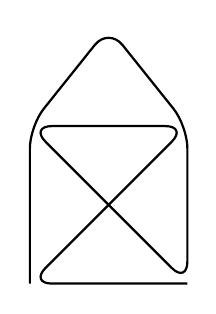
\begin{tikzpicture}
\tikz \draw[thick,rounded corners=8pt]
(0,0) -- (0,2) -- (1,3.25) -- (2,2) -- (2,0) -- (0,2) -- (2,2) -- (0,0) -- (2,0);
\end{tikzpicture}







\begin{tikzpicture}
\draw (-1.5,0) -- (1.5,0);
\draw (0,-1.5) -- (0,1.5);
\end{tikzpicture}




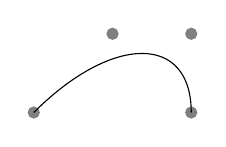
\begin{tikzpicture}
\filldraw [gray] (0,0) circle (2pt)
(1,1) circle (2pt)
(2,1) circle (2pt)
(2,0) circle (2pt);
\draw (0,0) .. controls (1,1) and (2,1) .. (2,0);
\end{tikzpicture}








\begin{tikzpicture}
\draw (-1.5,0) -- (1.5,0);
\draw (0,-1.5) -- (0,1.5);
\draw (0,0) circle (1cm);
\end{tikzpicture}





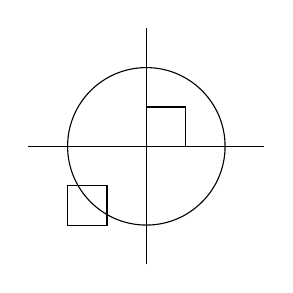
\begin{tikzpicture}
\draw (-1.5,0) -- (1.5,0);
\draw (0,-1.5) -- (0,1.5);
\draw (0,0) circle (1cm);
\draw (0,0) rectangle (0.5,0.5);
\draw (-0.5,-0.5) rectangle (-1,-1);
\end{tikzpicture}








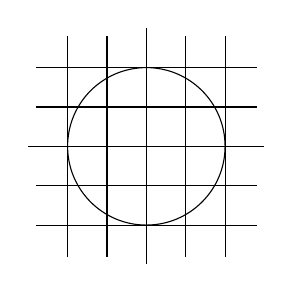
\begin{tikzpicture}
\draw (-1.5,0) -- (1.5,0);
\draw (0,-1.5) -- (0,1.5);
\draw (0,0) circle (1cm);
\draw[step=.5cm] (-1.4,-1.4) grid (1.4,1.4);
\end{tikzpicture}










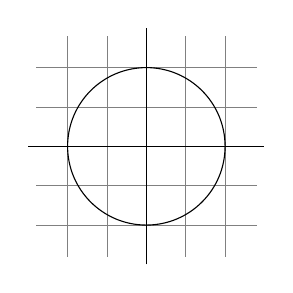
\begin{tikzpicture}
\draw[step=.5cm,gray,very thin] (-1.4,-1.4) grid (1.4,1.4);
\draw (-1.5,0) -- (1.5,0);
\draw (0,-1.5) -- (0,1.5);
\draw (0,0) circle (1cm);
\end{tikzpicture}







\begin{tikzpicture}[scale=3]
\draw[step=.5cm,gray,very thin] (-1.4,-1.4) grid (1.4,1.4);
\draw (-1.5,0) -- (1.5,0);
\draw (0,-1.5) -- (0,1.5);
\draw (0,0) circle (1cm);
\draw (3mm,0mm) arc (0:30:3mm);
\end{tikzpicture}









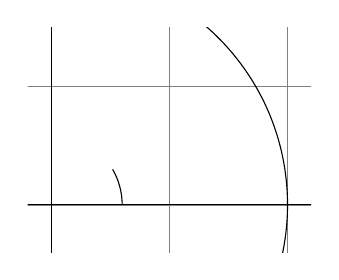
\begin{tikzpicture}[scale=3]
\clip (-0.1,-0.2) rectangle (1.1,0.75);
\draw[step=.5cm,gray,very thin] (-1.4,-1.4) grid (1.4,1.4);
\draw (-1.5,0) -- (1.5,0);
\draw (0,-1.5) -- (0,1.5);
\draw (0,0) circle (1cm);
\draw (3mm,0mm) arc (0:30:3mm);
\end{tikzpicture}









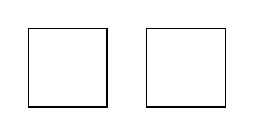
\begin{tikzpicture}
\def\rectanglepath{-- ++(1cm,0cm) -- ++(0cm,1cm) -- ++(-1cm,0cm) -- cycle}
\draw (0,0) \rectanglepath;
\draw (1.5,0) \rectanglepath;
\end{tikzpicture}






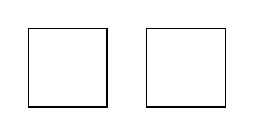
\begin{tikzpicture}
\def\rectanglepath{-- +(1cm,0cm) -- +(1cm,1cm) -- +(0cm,1cm) -- cycle}
\draw (0,0) \rectanglepath;
\draw (1.5,0) \rectanglepath;
\end{tikzpicture}






\begin{tikzpicture}[ultra thick]
\draw (0,0) -- (0,1);
\begin{scope}[thin]
\draw (1,0) -- (1,1);
\draw (2,0) -- (2,1);
\end{scope}
\draw (3,0) -- (3,1);
\end{tikzpicture}












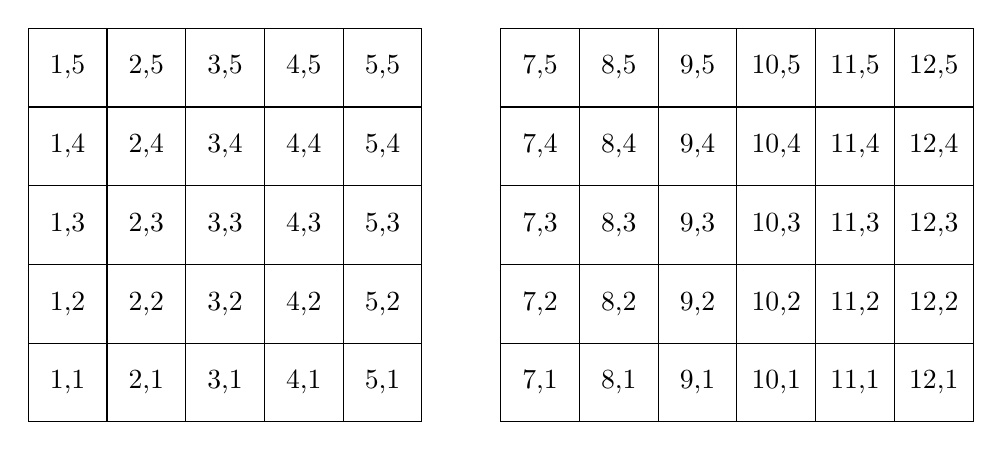
\begin{tikzpicture}
\foreach \x in {1,2,...,5,7,8,...,12}
\foreach \y in {1,...,5}
{
\draw (\x,\y) +(-.5,-.5) rectangle ++(.5,.5);
\draw (\x,\y) node{\x,\y};
}
\end{tikzpicture}




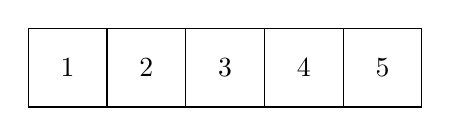
\begin{tikzpicture}
\def\rectanglepath{-- +(1cm,0cm) -- +(1cm,1cm) -- +(0cm,1cm) -- cycle}
\def\arrayOne{
	\foreach \x in {1,2,...,5}
	{
		\draw (\x,0) \rectanglepath;
		\draw (\x+.5,0.5) node{\x};
	}
}
\arrayOne
\end{tikzpicture}


\begin{center}
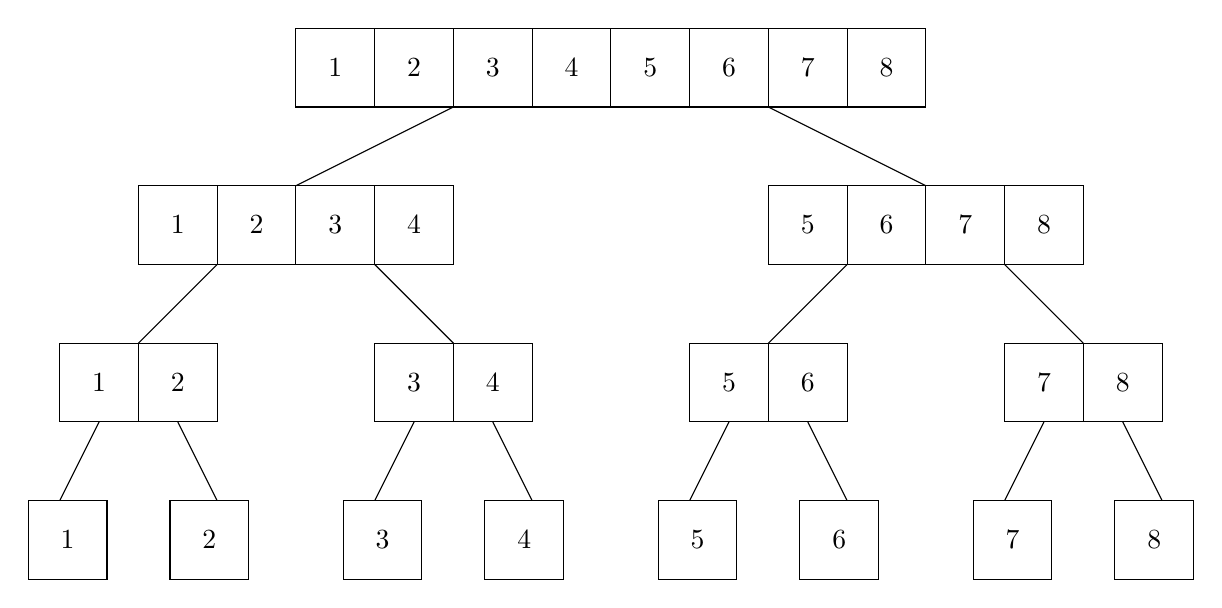
\begin{tikzpicture}
\def\rectanglepath{-- +(1cm,0cm) -- +(1cm,1cm) -- +(0cm,1cm) -- cycle}

\draw (3,0) -- (1,-1) ;
\draw (7,0) -- (9,-1) ;



\draw (0,-2) -- (-1,-3) ;
\draw (2,-2) -- (3,-3) ;

\draw (8,-2) -- (7,-3) ;
\draw (10,-2) -- (11,-3) ;



\draw (-1.5,-4) -- (-2,-5) ;
\draw (-.5,-4) -- (0,-5) ;

\draw (2.5,-4) -- (2,-5) ;
\draw (3.5,-4) -- (4,-5) ;

\draw (6.5,-4) -- (6,-5) ;
\draw (7.5,-4) -- (8,-5) ;


\draw (10.5,-4) -- (10,-5) ;
\draw (11.5,-4) -- (12,-5) ;

\foreach \x in {1,2,3,4,5,6,7,8}
{
	\draw (\x,0) \rectanglepath;
	\draw (\x+.5,0.5) node{\x};
}

\foreach \x in {1,2,3,4}
{
	\draw (\x-2,-2) \rectanglepath;
	\draw (\x-2+.5,0.5-2) node{\x};
}

\foreach \x in {5,6,7,8}
{
	\draw (\x+2,-2) \rectanglepath;
	\draw (\x+2+.5,0.5-2) node{\x};
}


\foreach \x in {1,2}
{
	\draw (\x-2-1,-2-2) \rectanglepath;
	\draw (\x-2-1+.5,0.5-2-2) node{\x};
}

\foreach \x in {1}
{
	\draw (\x-2-1-.4,-2-2-2) \rectanglepath;
	\draw (\x-2-1-.4+.5,0.5-2-2-2) node{\x};
}

\foreach \x in {2}
{
	\draw (\x-2-1+.4,-2-2-2) \rectanglepath;
	\draw (\x-2-1+.4+.5,0.5-2-2-2) node{\x};
}

\foreach \x in {3,4}
{
	\draw (\x-2+1,-2-2) \rectanglepath;
	\draw (\x-2+1+.5,0.5-2-2) node{\x};
}


\foreach \x in {3}
{
	\draw (\x-2+1-.4,-2-2-2) \rectanglepath;
	\draw (\x-2+1-.4+.5,0.5-2-2-2) node{\x};
}

\foreach \x in {4}
{
	\draw (\x-2+1+.4,-2-2-2) \rectanglepath;
	\draw (\x-2+1+.4+.5,0.5-2-2-2) node{\x};
}

\foreach \x in {5,6}
{
	\draw (\x+2-1,-2-2) \rectanglepath;
	\draw (\x+2-1+.5,0.5-2-2) node{\x};
}


\foreach \x in {5}
{
	\draw (\x+2-1-.4,-2-2-2) \rectanglepath;
	\draw (\x+2-1-.4+.5,0.5-2-2-2) node{\x};
}

\foreach \x in {6}
{
	\draw (\x+2-1+.4,-2-2-2) \rectanglepath;
	\draw (\x+2-1+.4+.5,0.5-2-2-2) node{\x};
}


\foreach \x in {7,8}
{
	\draw (\x+2+1,-2-2) \rectanglepath;
	\draw (\x+2+1+.5,0.5-2-2) node{\x};
}

\foreach \x in {7}
{
	\draw (\x+2+1-.4,-2-2-2) \rectanglepath;
	\draw (\x+2+1-.4+.5,0.5-2-2-2) node{\x};
}

\foreach \x in {8}
{
	\draw (\x+2+1+.4,-2-2-2) \rectanglepath;
	\draw (\x+2+1+.4+.5,0.5-2-2-2) node{\x};
}


\end{tikzpicture}
\end{center}




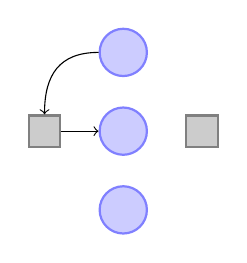
\begin{tikzpicture}
\tikzstyle{place}=[circle,draw=blue!50,fill=blue!20,thick,
inner sep=0pt,minimum size=6mm]
\tikzstyle{transition}=[rectangle,draw=black!50,fill=black!20,thick,
inner sep=0pt,minimum size=4mm]

\node[place] (waiting) {};
\node[place] (critical) [below of=waiting] {};
\node[place] (semaphore) [below of=critical] {};
\node[transition] (leave critical) [right of=critical] {};
\node[transition] (enter critical) [left of=critical] {};
\draw [->] (enter critical.east) -- (critical.west);
\draw [->] (waiting.west) .. controls +(left:5mm) and +(up:5mm)
.. (enter critical.north);
\end{tikzpicture}









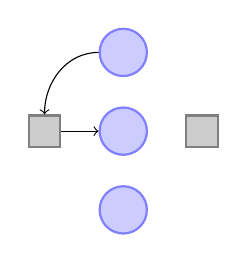
\begin{tikzpicture}
\tikzstyle{place}=[circle,draw=blue!50,fill=blue!20,thick,
inner sep=0pt,minimum size=6mm]
\tikzstyle{transition}=[rectangle,draw=black!50,fill=black!20,thick,
inner sep=0pt,minimum size=4mm]
\node[place] (waiting) {};
\node[place] (critical) [below of=waiting] {};
\node[place] (semaphore) [below of=critical] {};
\node[transition] (leave critical) [right of=critical] {};
\node[transition] (enter critical) [left of=critical] {};
\draw [->] (enter critical) to (critical);
\draw [->] (waiting) to [out=180,in=90] (enter critical);
\end{tikzpicture}





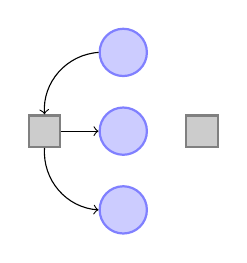
\begin{tikzpicture}
\tikzstyle{place}=[circle,draw=blue!50,fill=blue!20,thick,
inner sep=0pt,minimum size=6mm]
\tikzstyle{transition}=[rectangle,draw=black!50,fill=black!20,thick,
inner sep=0pt,minimum size=4mm]
\node[place] (waiting) {};
\node[place] (critical) [below of=waiting] {};
\node[place] (semaphore) [below of=critical] {};
\node[transition] (leave critical) [right of=critical] {};
\node[transition] (enter critical) [left of=critical] {};
\draw [->] (enter critical) to (critical);
\draw [->] (waiting) to [bend right=45] (enter critical);
\draw [->] (enter critical) to [bend right=45] (semaphore);
\end{tikzpicture}






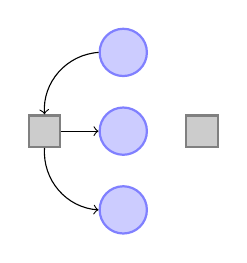
\begin{tikzpicture}
\tikzstyle{place}=[circle,draw=blue!50,fill=blue!20,thick,
inner sep=0pt,minimum size=6mm]
\tikzstyle{transition}=[rectangle,draw=black!50,fill=black!20,thick,
inner sep=0pt,minimum size=4mm]
\node[place] (waiting) {};
\node[place] (critical) [below of=waiting] {};
\node[place] (semaphore) [below of=critical] {};
\node[transition] (leave critical) [right of=critical] {};
\node[transition] (enter critical) [left of=critical] {}
edge [->] (critical)
edge [<-,bend left=45] (waiting)
edge [->,bend right=45] (semaphore);
\end{tikzpicture}















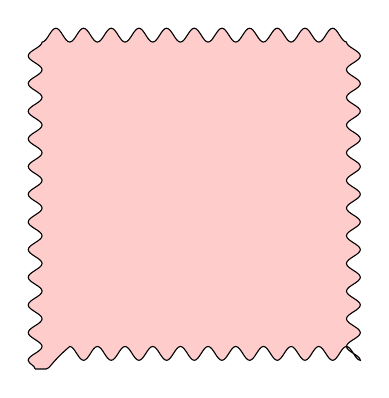
\begin{tikzpicture}
\filldraw[fill=red!20,decorate,decoration=snake] (0,0) rectangle (4,4);
\end{tikzpicture}








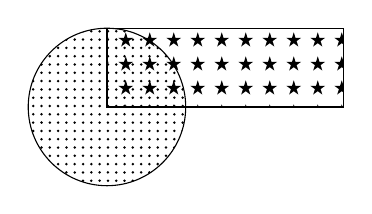
\begin{tikzpicture}
\draw[pattern=dots] (0,0) circle (1cm);
\draw[pattern=fivepointed stars] (0,0) rectangle (3,1);
\end{tikzpicture}







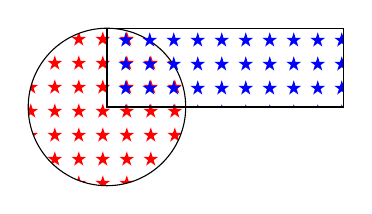
\begin{tikzpicture}
\draw[pattern color=red,pattern=fivepointed stars] (0,0) circle (1cm);
\draw[pattern color=blue,pattern=fivepointed stars] (0,0) rectangle (3,1);
\end{tikzpicture}







\begin{tikzpicture}
\def\mypath{(0,0) -- +(0,1) arc (180:0:1.5cm) -- +(0,-1)}
\fill [red] \mypath;
\pattern[pattern color=white,pattern=bricks] \mypath;
\end{tikzpicture}







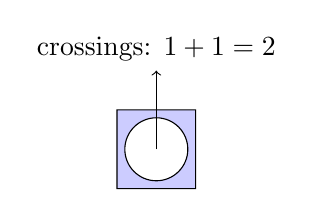
\begin{tikzpicture}
\filldraw[fill=blue!20,even odd rule]
(0,0) rectangle (1,1) (0.5,0.5) circle (0.4cm);
\draw[->] (0.5,0.5) -- +(0,1) [above] node{crossings: $1+1 = 2$};
\end{tikzpicture}









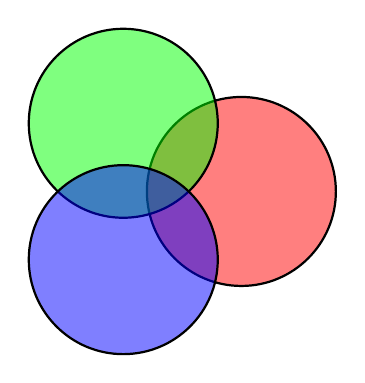
\begin{tikzpicture}[thick,fill opacity=0.5]
\filldraw[fill=red] (0:1cm) circle (12mm);
\filldraw[fill=green] (120:1cm) circle (12mm);
\filldraw[fill=blue] (-120:1cm) circle (12mm);
\end{tikzpicture}









\begin{tikzpicture}
\fill[red] (0,0) rectangle (3,2);
\node at (0,0) {\huge A};
\node[fill opacity=0.5] at (3,2) {\huge B};
\end{tikzpicture}











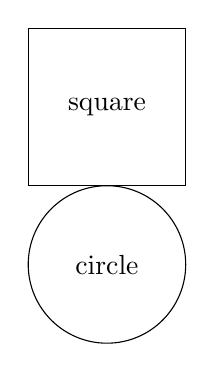
\begin{tikzpicture}
\draw (0,0) node[minimum size=2cm,draw] {square};
\draw (0,-2) node[minimum size=2cm,draw,circle] {circle};
\end{tikzpicture}






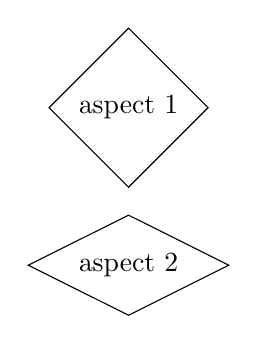
\begin{tikzpicture}
\draw (0,0) node[aspect=1,diamond,draw] {aspect 1};
\draw (0,-2) node[aspect=2,diamond,draw] {aspect 2};
\end{tikzpicture}









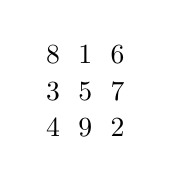
\begin{tikzpicture}
\tikzstyle{matrix of nodes}=[
execute at begin cell=\node\bgroup,
execute at end cell=\egroup;%
]
\matrix [matrix of nodes]
{
8 & 1 & 6 \\
3 & 5 & 7 \\
4 & 9 & 2 \\
};
\end{tikzpicture}







\begin{tikzpicture}
\tikzstyle{matrix of nodes}=[
execute at begin cell=\node\bgroup,
execute at end cell=\egroup;,%
execute at empty cell=\node{--};%
]
\matrix [matrix of nodes]
{
8 & 1 & \\
3 & & 7 \\
& & 2 \\
};
\end{tikzpicture}










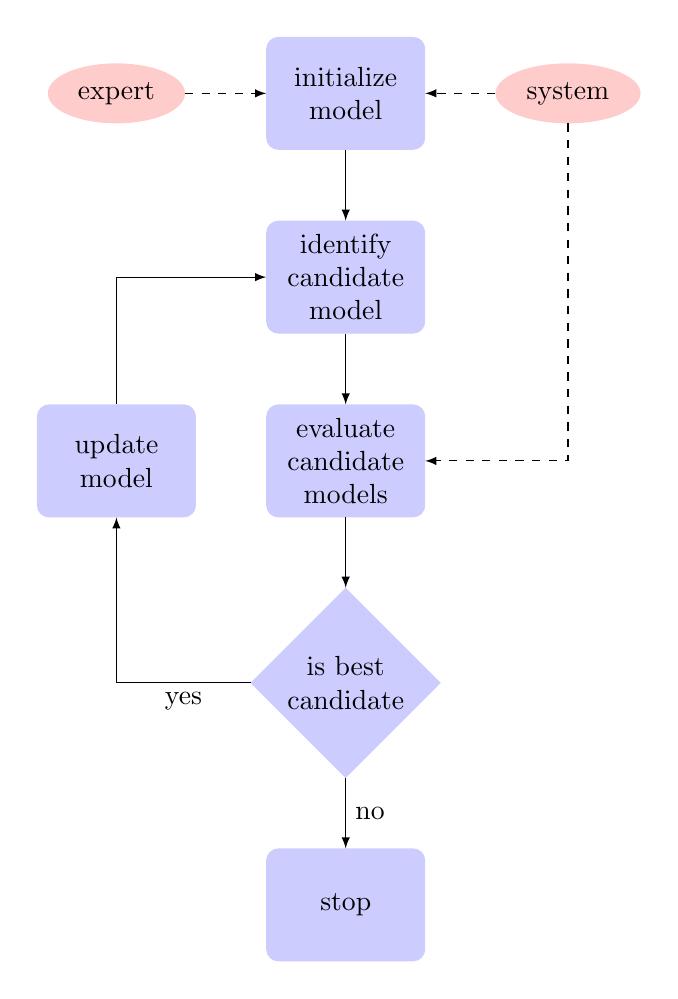
\begin{tikzpicture}[auto]
\tikzstyle{decision} = [diamond, draw=blue!20, thick, fill=blue!20,
text width=4.5em, text badly centered, inner sep=1pt]
\tikzstyle{block} = [rectangle, draw=blue!20, thick, fill=blue!20,
text width=5em, text centered, rounded corners, minimum height=4em]
\tikzstyle{line} = [draw, thick, -latex’,shorten >=2pt];
\tikzstyle{cloud} = [draw=red!20, thick, ellipse,fill=red!20, minimum height=2em];
\matrix [column sep=7mm,row sep=9mm]
{
% row 1
\node [cloud] (expert) {expert}; &
\node [block] (init) {initialize model}; &
\node [cloud] (system) {system}; \\
% row 2
& \node [block] (identify) {identify candidate model}; & \\
% row 3
\node [block] (update) {update model}; &
\node [block] (evaluate) {evaluate candidate models}; & \\
% row 4
& \node [decision] (decide) {is best candidate}; & \\
% row 5
& \node [block] (stop) {stop}; & \\
};
%\tikzstyle{every path}=[line]
\draw[->,>=latex] (init) -- (identify);
\draw[->,>=latex] (identify) -- (evaluate);
\draw[->,>=latex] (evaluate) -- (decide);
\draw[->,>=latex] (update) |- (identify);
\draw[->,>=latex] (decide) -| node [near start] {yes} (update);
\draw[->,>=latex] (decide) -- node [midway] {no} (stop);
\draw[->,>=latex] [dashed] (expert) -- (init);
\draw[->,>=latex] [dashed] (system) -- (init);
\draw[->,>=latex] [dashed] (system) |- (evaluate);
\end{tikzpicture}




\newpage

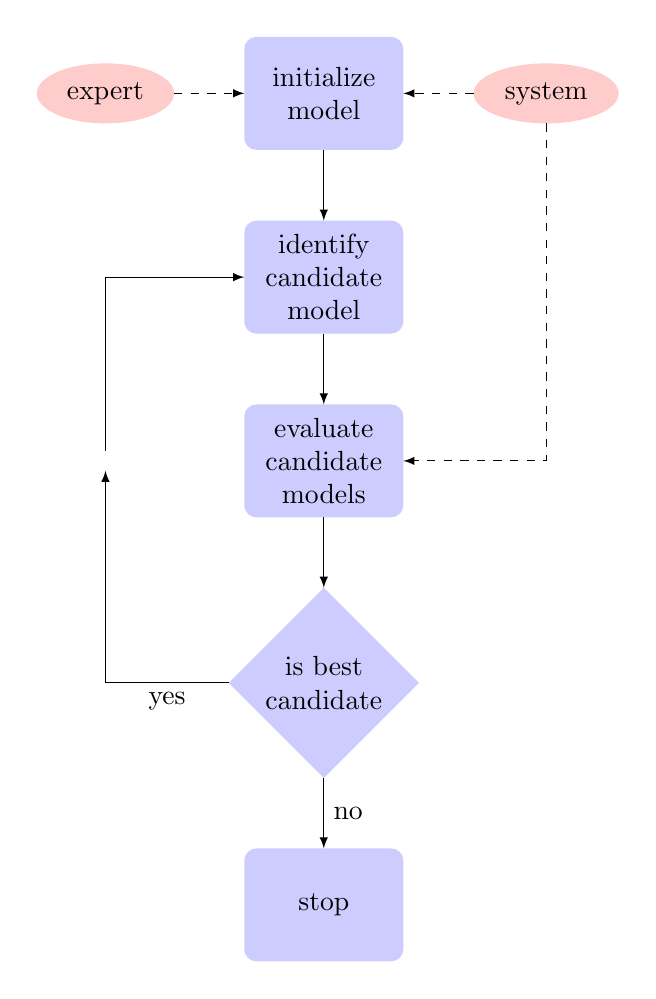
\begin{tikzpicture}[auto]
\tikzstyle{decision} = [diamond, draw=blue!20, thick, fill=blue!20,
text width=4.5em, text badly centered, inner sep=1pt]
\tikzstyle{block} = [rectangle, draw=blue!20, thick, fill=blue!20,
text width=5em, text centered, rounded corners, minimum height=4em]
\tikzstyle{line} = [draw, thick, -latex’,shorten >=2pt];
\tikzstyle{cloud} = [draw=red!20, thick, ellipse,fill=red!20, minimum height=2em];
\matrix [column sep=7mm,row sep=9mm]
{
% row 1
\node [cloud] (expert) {expert}; &
\node [block] (init) {initialize model}; &
\node [cloud] (system) {system}; \\
% row 2
& \node [block] (identify) {identify candidate model}; & \\
% row 3
\node  (update) {}; &
\node [block] (evaluate) {evaluate candidate models}; & \\
% row 4
& \node [decision] (decide) {is best candidate}; & \\
% row 5
& \node [block] (stop) {stop}; & \\
};
%\tikzstyle{every path}=[line]
\draw[->,>=latex] (init) -- (identify);
\draw[->,>=latex] (identify) -- (evaluate);
\draw[->,>=latex] (evaluate) -- (decide);
\draw[->,>=latex] (update) |- (identify);
\draw[->,>=latex] (decide) -| node [near start] {yes} (update);
\draw[->,>=latex] (decide) -- node [midway] {no} (stop);
\draw[->,>=latex] [dashed] (expert) -- (init);
\draw[->,>=latex] [dashed] (system) -- (init);
\draw[->,>=latex] [dashed] (system) |- (evaluate);
\end{tikzpicture}












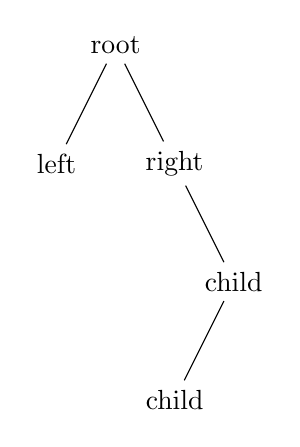
\begin{tikzpicture}
\node {root}
	child {node {left}
	}
	child {node {right}
		child[missing] {node {child}}
		child {node {child}
			child {node {child}}
			child[missing] {node {child}}
		}
	};
\end{tikzpicture}






\begin{tikzpicture}
\node {root} [grow=right]
	child {node {left}
	}
	child {node {right}
		child[missing] {node {child}}
		child {node {child}
			child {node {child}}
			child[missing] {node {child}}
		}
	};
\end{tikzpicture}








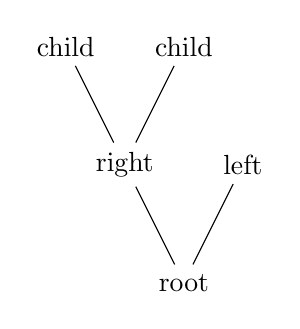
\begin{tikzpicture}
\node {root} [grow=up]
child {node {left}}
child {node {right}
child {node {child}}
child {node {child}}
};
\end{tikzpicture}








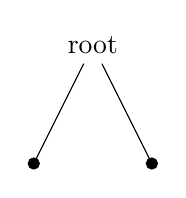
\begin{tikzpicture}
\node {root}
child {[fill] circle (2pt)}
child {[fill] circle (2pt)};
\end{tikzpicture}






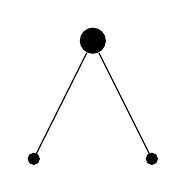
\begin{tikzpicture}
\node[circle,fill=black,minimum width=8pt] {}
child {[fill] circle (2pt)}
child {[fill] circle (2pt)};
\end{tikzpicture}







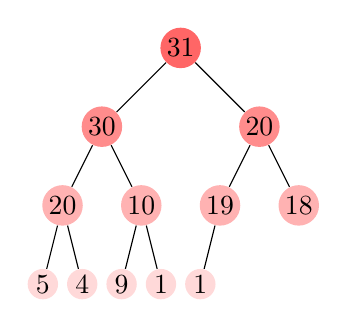
\begin{tikzpicture}[level distance=10mm]
\tikzstyle{every node}=[fill=red!60,circle,inner sep=1pt]
\tikzstyle{level 1}=[sibling distance=20mm,
set style={{every node}+=[fill=red!45]}]
\tikzstyle{level 2}=[sibling distance=10mm,
set style={{every node}+=[fill=red!30]}]
\tikzstyle{level 3}=[sibling distance=5mm,
set style={{every node}+=[fill=red!15]}]
\node {31}
child {node {30}
	child {node {20}
		child {node {5}}
		child {node {4}}
	}
	child {node {10}
		child {node {9}}
		child {node {1}}
	}
}
child {node {20}
	child {node {19}
		child {node {1}}
		child[fill=none] {edge from parent[draw=none]}
	}
	child {node {18}}
};
\end{tikzpicture}










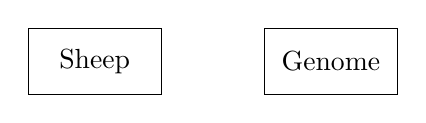
\begin{tikzpicture}[node distance=3cm]
\node[entity] (sheep) {Sheep};
\node[entity] (genome) [right of=sheep] {Genome};
\end{tikzpicture}









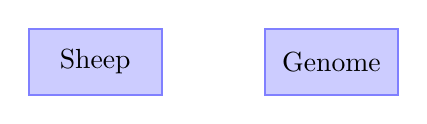
\begin{tikzpicture}[node distance=3cm]
\tikzstyle{every entity}=[draw=blue!50,fill=blue!20,thick]
\node[entity] (sheep) {Sheep};
\node[entity] (genome) [right of=sheep] {Genome};
\end{tikzpicture}










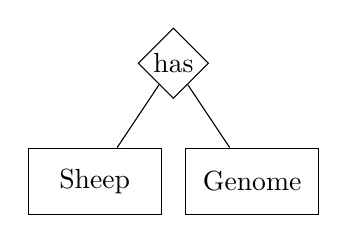
\begin{tikzpicture}
\node[entity] (sheep) at (0,0) {Sheep};
\node[entity] (genome) at (2,0) {Genome};
\node[relationship] (rel) at (1,1.5) {has};
\draw (rel) -- (sheep);
\draw (rel) -- (genome);
\end{tikzpicture}








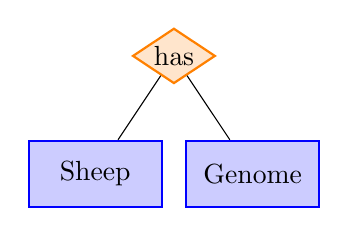
\begin{tikzpicture}
\tikzstyle{every entity}=[fill=blue!20,draw=blue,thick]
\tikzstyle{every relationship}=[fill=orange!20,draw=orange,thick,aspect=1.5]
\node[entity] (sheep) at (0,0) {Sheep};
\node[entity] (genome) at (2,0) {Genome};
\node[relationship] (rel) at (1,1.5) {has};
\draw (rel) -- (sheep);
\draw (rel) -- (genome);
\end{tikzpicture}








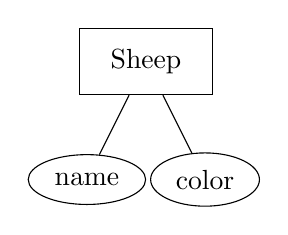
\begin{tikzpicture}[node distance=3cm]
\node[entity] (sheep) {Sheep}
child {node[attribute] {name}}
child {node[attribute] {color}};
\end{tikzpicture}





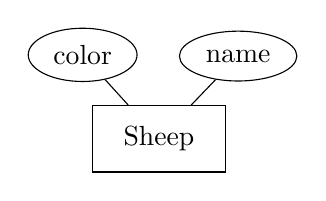
\begin{tikzpicture}
\tikzstyle{every pin edge}=[draw]
\node[entity,
pin={[attribute]60:name},
pin={[attribute]120:color}] 
{Sheep};
\end{tikzpicture}








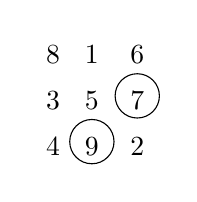
\begin{tikzpicture}
\matrix [matrix of nodes]
{
8 & 1 & 6 \\
3 & 5 & \node[black]{7}; \draw(0pt,5pt) circle(8pt);\\
4 & \node[black]{9}; \draw(0pt,5pt) circle(8pt); & 2 \\
};
\end{tikzpicture}









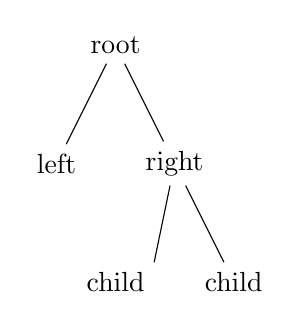
\begin{tikzpicture}
\node {root}
child {node {left}}
child {node {right}
child[child anchor=north east] {node {child}}
child {node {child}}
};
\end{tikzpicture}


















\begin{tikzpicture}
\foreach \x in {0,1,2,3}
\draw (\x,0) circle (0.2cm);
\end{tikzpicture}







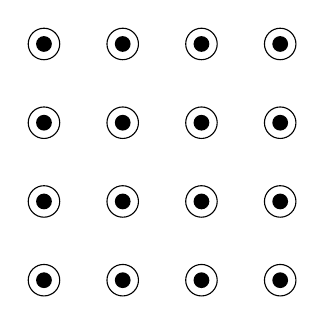
\begin{tikzpicture}
\foreach \x in {0,1,2,3}
	\foreach \y in {0,1,2,3}
	{
		\draw (\x,\y) circle (0.2cm);
		\fill (\x,\y) circle (0.1cm);
	}
\end{tikzpicture}
















\end{document}